\section{Highscore database}
Som proof-of-concept er der udviklet en applikation til PC'en som kommunikerer med LC3 Computeren over en seriel forbindelse for at lagre highscores i en database, applikationen er skrevet i C\#.

\begin{wrapfigure}{r}{0.4\textwidth}
  \begin{center}
    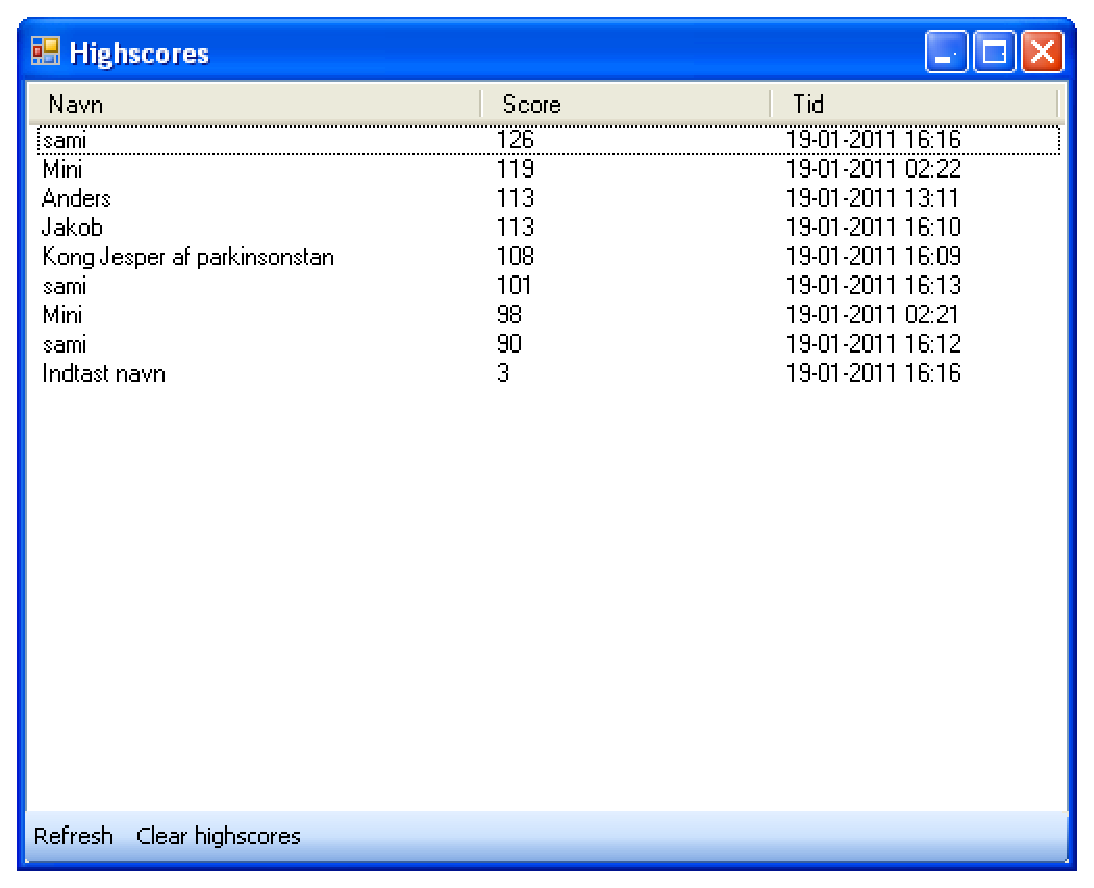
\includegraphics[width=0.38\textwidth]{billeder/HighscoreBoard}
  \end{center}
  \caption{Screenshot af highscore applikationen}
\end{wrapfigure}

Applikationen opretter en tråd hvis formål er at poole for data på seriel forbindelsen, af den årsag er det heller ikke muligt at køre andre programmer samtidig som bruger seriel forbindelsen. Når en linje modtages med scoren oprettes et "Game Over" vindue hvor det er muligt at skrive sig på highscore listen, spillet er imens på pause indtil karakteren 's' (for start) sendes tilbage over serial forbindelsen af highscore applikationen når highscoren er gemt hvorefter spillet nulstiller og starter forfra.

Applikationen benytter en database til at lagre highscores, det er valgt at benytte en sqlite\footnote{For yderligere information om SQLite databaser se http://sqlite.org} database da denne danner baggrund for en simpel og hurtig database gemt i en enkelt fil i modsætning til alternativer som f.eks. MySQL som benytter kræver en database server.

En simpel tabel er oprettet til at indeholde highscore listen, bemærk at \texttt{submitted\_at} angiver tiden for oprettelsen af scoren i unix tid\footnote{Unix tid er angivet i antal sekunder siden d. 1. Januar 1970} formatet.

%\billede{!htbp}{0.3}{HighscoreBoard}{Screenshot af highscore applikationen}

\lstset{language=SQL}
\begin{lstlisting}
CREATE TABLE highscore(
	name varchar(200),
	score int,
	submitted_at int
);
\end{lstlisting}

% Henvis til OOAD og DB